\documentclass[]{usiinfbachelorproject}

\captionsetup{labelfont={bf}}

\author{Simone D'Avico}

\title{A Dynamic Monitoring Component of a Data Flow testing tool}
\subtitle{}
\versiondate{\today}

\includeonly{./Sections/introduction_alt,./Sections/goalandchallenges,
./Sections/relatedwork,./Sections/tool,./Sections/validation,./Sections/conclusion}

\begin{committee}
%With more than 1 advisor an error is raised...: only 1 advisor is allowed!
\advisor[Universit\`a della Svizzera Italiana, Switzerland]{Prof.}{Mauro}{Pezz\'e}
%You can comment out  these lines if you don't have any assistant
\assistant[Universit\`a della Svizzera Italiana, Switzerland]{ }{Mattia}{Vivanti}
%\assistant[Universit\`a della Svizzera Italiana, Switzerland]{Title}{AssistantName2}{AssistanSurname2}
\end{committee}

\abstract {

This bachelor project focuses on the design of an automatic tool for data flow coverage computation. Data flow coverage criteria are a promising technique that tracks covered data flow relations in the code to assess the quality of a test suite and to steer test case generation. Data flow criteria have been theorized to be more effective than simpler criteria like statement and branch coverage, but as of today their applicability is limited by the complexity required to compute the coverage measure, that in the lack of automatic tools have to be done manually. 

In this project I designed, developed and tested a component of  an automatic data flow testing tool called \datec, to provide a new efficient tool for computing data flow coverage for java programs.
More specifically, I focused on the implementation of a dynamic runtime monitor component for the coverage computation, and then I carried on the validation activity of the tool verifying its efficiency and correctness.

The result of the project is a efficient a reliable tool, that I am going to release online to help researchers and practitioners experimenting with data flow criteria, since up to now, \datec~is the only available data flow testing tool for object oriented systems.


%Even though they have been discussed in literature for a long time, they are rarely used in practice. Their applicability is limited mostly by their complexity

% and the lack of automated tools for data-flow testing. The main goal of this bachelor project is  to address this concern by developing and evaluating a component for a data-flow testing tool called \datec. More specifically, I focused on the implementation of a dynamic monitor for runtime data-flow coverage computation; on a second time, I verified the tool's efficiency and the correctness of the results with a number of test cases. Results show that the number of test cases required in order to effectively apply data-flow testing  is much greater than the number of test cases required to measure according to more classical criteria, like functional or simpler statement testing criteria. 

}

\newcommand{\datec}{DaTeC}
\newcommand{\disl}{DiSL}
\usepackage{pifont,calc,xcolor}
\usepackage{listings}
\usepackage{parcolumns}
\definecolor{verylightgray}{gray}{0.85}
\newlength\lsthorizontalpadding
\setlength\lsthorizontalpadding{3pt}
\newcommand*\lstnumberstyle{\ttfamily\scriptsize}
\newlength\lstnumbersep
\setlength\lstnumbersep{10pt}
\newlength\lstnumberwidth
\setlength\lstnumberwidth{\widthof{\lstnumberstyle00}+\lstnumbersep+\lsthorizontalpadding}

\usepackage{float}
\restylefloat{table}

\lstset{
    ,basicstyle=\ttfamily%
    ,breaklines=true%
    ,tabsize=4%
    ,showstringspaces=false%
    ,numbers=left%
    ,numbersep=\lstnumbersep%
    ,numberstyle=\lstnumberstyle%
    ,framesep=0pt%
    %,backgroundcolor=\color{verylightgray}%
    ,xleftmargin=\lstnumberwidth%
    ,framexleftmargin=\lsthorizontalpadding%
    ,xrightmargin=\lsthorizontalpadding%
    ,framexrightmargin=\lsthorizontalpadding%
    ,postbreak=\ding{229}\space%
    ,captionpos=b
}

\lstnewenvironment{jcode}[1][]{\lstset{language=Java,#1}}{}

\begin{document}
\maketitle

\section{Introduction}\label{introduction}

\paragraph{}
Software testing is the prevailing activity for software quality assurance in 
most industrial settings. Software testing consists in generating a set of representative inputs 
and oracles, which are exercised in order to compare the outputs against the specifications to assess 
correctness. 
One of the intrinsic challenges of testing is to evaluate the \textit{adequacy} 
of a test suite, that is, establishing whether a test suite exercises 
the software to a sufficient extent, or has to be augmented with the 
definition of new test cases. Deciding whether a software has been tested enough is challenging: Ideally, a test suite should be 
considered adequate when able to reveal all the faults in the program 
under test, but without knowing in advance the faults present in the 
code (that is the information that you are investigating with testing), it is impossible to precisely evaluate the thoroughness of a test suite. 
Thus, researchers proposed different techniques that approximate the 
thoroughness of a test suite, using other sources of information than the number of detected faults.

\paragraph{}
These approaches are either based on the specifications or on the 
structure of the software under test. \textit{Functional techniques} 
approximate the thoroughness of a test suite by measuring the relative 
amount of exercised functionality with respect to all the 
functionalities written in the specifications, while \textit{structural 
techniques} look at the fraction of executed code entities with respect 
to their totality. 

\paragraph{}
In this project I focus on \textit{structural techniques}. These techniques starts from the observation that to effectively reveal a 
fault, a test suite has to execute the code entities that contain the bug and lead to a failure. 
Thus, structural adequacy criteria consider a test suite to be adequate only is it is able to exercise the majority of 
code entities in the program under test. These code entities could be 
simple elements like statements and branches, or more complex entities 
such as paths of the control flow graph. 

\paragraph{}
In the last decades control flow-based criteria, that are criteria that requires the execution of elements of the control flow graph, such as statements and 
branches, got more and more popular and nowadays they are becoming a standard in many companies and in open source projects. This class of criteria has been the first one to be acknowledged by practitioners, and a crucial factor in their establishment has been the diffusion of robust and efficient tools to automate the coverage computation. 

\paragraph{}
Besides control flow-based criteria, a promising class of criteria is 
data flow ones. Data flow criteria use data flow analysis techniques to identify possible data propagation and usage in the program under test, and then approximate the thoroughness of a test suite as the number of covered data relationships at runtime (for instance, pairs of definitions and uses of the same variables). The rational of data flow criteria is that to reveal a fault, is necessary not only to execute the faulty line of the code that perform a faulty computation, but also a subsequent use of that value that lead to a detectable failure. 

\paragraph{}
However, while data flow criteria have been suggested to be more effective than control flow ones, they are rarely used in practice.
The major problem is that testers have to put very high effort in checking data flow coverage of test cases. Intuitively, it is more difficult to check if a test case exercised a variable definition as well as a use of that variable at another place, rather than just having to check the coverage of single statements and branches. This emphasizes the importance of automated tool for coverage computation --- however, most existing coverage tools target either statement or branch coverage, not tracking data flow coverage.

\paragraph{}
The production of tools which can automate data flow coverage computation 
and guarantee robustness and efficiency as it already happens for control flow 
criteria is fundamental in the interest of diffusion and study of data flow testing. To this end, in my bachelor project I designed and implemented a component for the computation of 
the achieved data flow coverage of a test suite by means of dynamic analysis at software execution time.

\paragraph{}
In this report, I introduce some background concepts necessary in order to understand the purpose of the tool I implemented, and I describe the tool's implementation and evaluation. Section \ref{goal} introduces the goal and the challenges of the project; Section \ref{related} introduces some concepts regarding data flow analysis and criteria; Section \ref{tool} addresses the tool's implementation, and Section \ref{validation} discusses the evaluation; finally, Section  \ref{conclusions} concludes.





\section{Goal and Challenges}\label{goal}

%Goal: fare sto tool 
%challenges: performance, problemi tecnici, problemi nel testarlo dato 
%che verificare a mano le coppie è un lavoro lunghissimo. 
In my bachelor project I designed, implemented and tested a dynamic monitor component for a data flow testing tool.
The tool's purpose is the computation of the fraction of definition-use pairs covered during the execution 
of a test suite. To do so, the tool in question depends on two different components. The first one 
performs a static analysis on the program under test to compute the \textit{coverage domain}, that is, 
all the possible definition-use pairs present in the software. The second component then performs dynamic 
analysis during the execution of a test suite to check how many of the detected definition-use pairs 
were covered by the test suite.

%this is the goal
\paragraph{}
My work focused on the design, implementation and testing of the latter component: I was provided with 
a data flow analysis tool for Java called \datec \cite{Denaro}, and I was asked to implement the 
component that computes how many of the definition-use pairs identified by \datec\ were covered 
during the execution of a test suite. Figure~\ref{schema} summarizes the components and outputs of the data flow testing tool.

%these are the challenges:
%keep modularity
\paragraph{}
The main goal of this project is to complete the implementation of the data flow testing tool, still ensuring a high degree of modularity and flexibility. The coverage computation component has to interface with the output of \datec, but has to be independent and flexible to changes done to the static analysis component that, being a research tool, is frequently modified.

%acquisition of knowledge
\paragraph{}
The first challenge that I had to face was the acquisition of the theoretical knowledge about data flow
testing,  as these topics are not usually covered during Bachelor studies. The second one was the study
of the already implemented component for static analysis, as I had to interface my implementation with 
the output produced by the static analysis.

%choosing instrumentation tool
%after explanation of the tool, add modularity concern
\paragraph{}
\datec's static analysis component is not the only component my tool has to interface with, as dynamic coverage analysis requires 
a way to trace method entry and exit points as well as variable definitions and uses at runtime. To this extent, one challenge had been  
to choose a technique to perform code instrumentation from a range of candidate ones, evaluating them from their functionalities, performance,  usage complexity and compatibility with a modular design. 

Another challenge of integrating a new implementation with an existing one is the definition of a common data format. In this context, static and dynamic information are computed using different techniques and tools, using different formats and level of abstraction. Therefore, another challenge was the definition of a strategy to manipulate these formats to achieve compatibility without actually coupling the implementations. 

 \begin{figure}[h]
   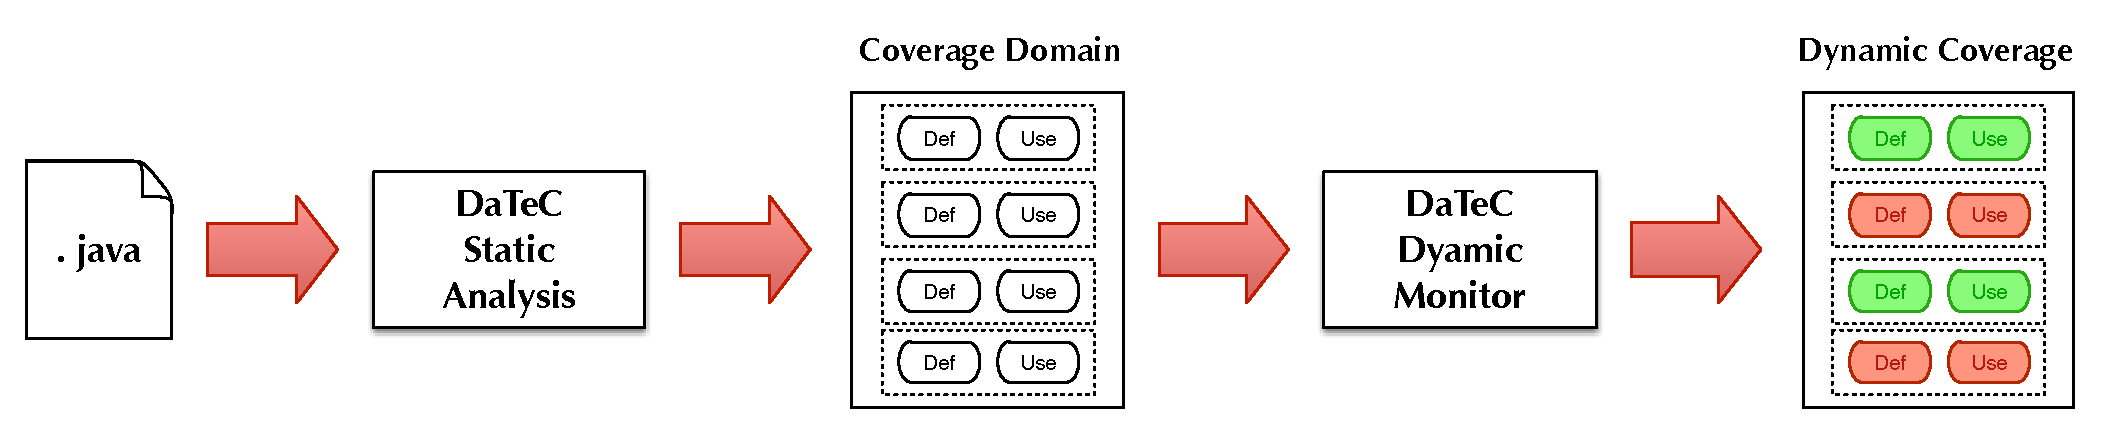
\includegraphics[width=\textwidth]{./Images/tool_highlevel.pdf}
   \caption{Exemplification of the components' role in coverage computation}
  \label{schema}
 \end{figure}

%last challenges: performance and verification
\paragraph{}
The last concern was performance and scalability, as projects could come with hundreds of test cases that produces hundreds of executions. Thus, it is important to limit the overhead of the tool to keep the execution time of big test suites within a reasonable amount of time. This is particularly challenging due to the fact that instrumentation is expensive, and that big projects have thousands of data flow elements to check.

The huge amount of analyzed data also posed a challenge in regards to the evaluation and 
verification process of the tool, as manually computing DU coverage is feasible 
only for smaller test suites, but still hard and time consuming. 

\section{Data Flow Analysis and Criteria}\label{related}

\subsection{Overview}

Data Flow models  were originally developed in the field of compiler
construction. They focus on transmission of information through program variables, and emphasize 
relations involving transmission of informations. The most fundamental class of data flow model
study the propagation of definitions of values (\textit{reaching definitions analysis}), striving to capture the flow of data through a program. 

\paragraph{}
Such analysis techniques and models have been used lately in the context of software testing. In particular, they 
have been used to approximate the thoroughness of a test suite exploiting the associations between definitions and uses of the same variable. This approach should raise the probability of revealing a fault in the program, unveiling bad computations by enforcing the use of all defined variables. Moreover, it provides a complementary view to the classical structural approaches, emphasizing relations involving transmission of informations. 


\subsection{Definition-use pairs}
A definition-use pair (DU pair) is defined as a pair of two program points, where the definition is the point in which a variable is assigned a
new value and the use is the point where that value is extracted. A definition of a variable is paired with the use of the same variable only if exists at least one path where the definition can reach the use without being overwritten (killed). Such a path is called \textit{definition-clear path}. More formally: \vspace{2mm}

\begin{center}
\begin{minipage}{0.9\textwidth}
\textbf{Definiton: }\textit{A DU pair can exist for some variable \textit{v}, iff there is at least one 
definition-clear path from the point of definition $v_d$ to the point of use $v_u$. In this case, we can
define $v_d$ as a \textit{reaching definition} at $v_u$.}  
\end{minipage}
\end{center}
%This concept is 
%important in the context of practical algorithms to compute DU pairs: as it is 
%not feasible to search all paths in the program control flow graph, they 
%summarize the reaching definitions at a node over all the paths reaching that 
%node. It is possible to efficiently compute reaching definitions of node 
%\textit{n} having an immediate predecessor \textit{p} by following simple rules:
%
%\begin{itemize}
%  \item If \textit{p} can assign a value to a variable \textit{v}, than 
%  definition $v_p$ reaches \textit{n}. $v_p$ is generated at \textit{p}.
%  \item If a definition $v_d$ of \textit{v} reaches a predecessor node 
%  \textit{p}, and if $v_d$ is not killed, then the definition is propagated from 
%  \textit{p} to \textit{n}.
%\end{itemize}
%
%From these two observations, it is possible to define a set of equations to be 
%exploited in algorithms to efficiently perform data flow analysis.

\subsection{Data Flow Testing Criteria}\label{criteria}

Definition-use pairs can be used to define different test requirements and coverage criteria, in order to approximate the thoroughness of a given test suite.
Herman \cite{Herman} defined one of the earliest and simplest criteria, the \textit{all definitions/uses coverage adequacy criterion}. This criterion requires pairing each variable definition with at least one use, or viceversa. The performed coverage is described by the formula 

\begin{center}
  $C_{defs} = \frac{\text{number of covered definitions}}
  {\text{number of definitions}}$
\end{center}

Later, several data  flow testing criteria where formally defined by Rapps and Weyuker first \cite{Rapps}, and Clarke et al. in a second time \cite{Clarke}. These criteria require the coverage of definition-use pairs in different ways, featuring different levels of complexity.
As of today, the most popular data flow criteria is the \textit{all DU pairs adequacy criterion}, which 
requires each DU pair to be covered in at least one program execution. In this 
case, the test suite will be adequate iff for each DU \textit{du} pair there is at least one 
test case covering \textit{du}. The corresponding coverage measure is the 
proportion of covered pairs: 

\begin{center}
  $C_{DU pairs} = \frac{\text{number of covered DU pairs}}{\text{number of DU pairs}}$
\end{center}
%
There is also an extension of the all DU pairs coverage, called \textit{all DU paths adequacy 
criterion}. This criterion requires each non-looping DU path to be traversed at 
least once, in order to cover all possible ways of pairing definitions and uses. 
This criterion can sometimes reveal faults by exercising a path on which a 
definition of the variable is missing.  Listing \ref{du_criteria} better exemplifies the different approaches of the DU pairs criterion and the all DU paths criterion:

\begin{minipage}{0.5\textwidth}
\begin{jcode}[caption={Simple branching code}, label={du_criteria}]
public void foobar(){
  int a = 0;
  int b = Random.nextInt(2);
  if(b%2 == 0) somethingEven();
  else somethingOdd();
  int c = a;
}
\end{jcode} 
\end{minipage}
\begin{minipage}{0.5\textwidth}
While the all DU pairs criterion would require only the coverage of the pair 
described by the definition of \texttt{a} at line 2 and its use at line 6 independently of the subsequent 
branch, the all DU paths criterion requires that both the \texttt{if} and the \texttt{else} 
paths are exercised.
\end{minipage}

\paragraph{}
In this case, a test suite is considered adequate iff, for each non-looping 
path \textit{dp} of the program, there is at least one test case that covers a path that 
includes \textit{dp}. The coverage measure deriving from this criterion is:

\begin{center}
  $C_{DU paths} = \frac{\text{number of exercised non-looping DU paths}}
  {\text{number of non-looping paths}}$
\end{center}
%
Unfortunately, although in the average case the number of DU paths is quite 
modest, it can be exponential in the size of the program in the worst case, 
especially when it contains many control paths. In many cases, this criterion is 
too costly. 

\paragraph{}
Under these premises, we decided to focus on the all-DU pairs adequacy criterion, as it is the most popular one
and features an average level of complexity.

\subsection{Limitations}
%può andar bene ma contestualizza. Questo è un problema, che in qualche modo ho visto ppoi durante l'implementazione.
Being a static analysis technique, data flow analysis is an approximation of 
the program behavior at runtime. As such, it suffers from imprecision when 
dealing with dynamic access to storage or dynamically allocated storage. For 
example, in the case of arrays, it is generally not possible to determine if two 
accesses refer to the same location (see Listing \ref{aliases}). The same problem occurs when dealing with 
references, as two different names could refer to the same storage location. 

\begin{center}
\begin{minipage}{0.6\textwidth}
\begin{jcode}[caption={Are these two lines a DU pair?}, label={aliases}]
a[i] = 2
b = a[j]
\end{jcode} 
\end{minipage}
\end{center}
%
How to treat these aliases depends on the use of the analysis results. In some 
cases, some degree of approximation in dealing with this kind of problem may be 
preferable to very expensive analysis. I observed this problem in my implementation because, 
in the case of arrays, \datec\ treats every write to an index as a definition of the array, and each access to an 
index as a use. 

\paragraph{}
Another limitation of data flow criteria is their applicability: even though 
data flow test techniques have been suggested to be effective, they are limited 
by the difficulty of generation of test suites which can guarantee good 
coverage, and a not so clear understanding of the scalability of the technique in 
practical approaches. All these factors lead to a lack of tools that apply data 
flow coverage techniques. %\datec\ and Coverlipse\footnote{\url{http://coverlipse.sourceforge.net.}}
%are an example, but they suffer from the problems mentioned above.


%data flow originariamente definito per programmi procedurali, è stato poi esteso a OO. In questo contesto le coppie non solo possono apparire all'interno di uno stesso metodo, ma anche in metodi diversi, richiedendo casi di test che stimolano in maniera più approfondita una classe rispetto a criteri basati su control flow. 
%In contesto OO si parla solitamente di coppie intra-metodo, inter-metodo e intra classe.Definizioni.
%le coppie intra classe sono le più interessanti per il test object oriented e sono quelle sulle quali si concentra datec e conseguentemente il mio tool.
\subsection{Data flow testing of classes}
%performed by Harrold and Rothermel \cite{Harrold} 
Data Flow testing was originally defined for procedural programs. Later studies \cite{Buy},\cite{Harrold},\cite{Pezze2008} showed that data flow testing is particularly suitable for object-oriented programming because object oriented logic focus more on data interactions and dependencies than complex intra procedural logic. In that context, DU pairs can occur not only within the same method, but also across methods, requiring test cases that exercise classes more meticulously than control flow criteria. More specifically, for object oriented data flow we can distinguish between \textit{intra-method} and \textit{inter-method} DU pairs:
%or \textit{intra-class}

 \begin{itemize}
   \item \textit{intra-method} DU pairs: the definition and use of a variable occur within the same method, and
   the pair is exercised during a single invocation of the method;
   \item \textit{inter-method} DU pairs: The definition and the use of the same variable are in different methods,
    and the path from the definition to the use can be found by following the method invocations in the control
    flow graph;
 \end{itemize}

Harrold and Rothermel \cite{Harrold} extended this approach by considering the data flow through the fields of an object in case that the public method of a class are called in arbitrary order. This is particularly important for isolated classes in which the behavior of a method may depend on the fields' current state. As an example, consider class \texttt{TicketClerk} (Figure \ref{ticketclerk}):

\begin{figure}[t]
  \begin{minipage}{0.5\textwidth}
    \begin{jcode}
public class TicketClerk {
  private float payedAmount;
  
  public TicketClerk(){
    payedAmount = 0;
  }
  
  public void pay(float amount) {
    payedAmount += amount;
  }
  
  ...
}      
    \end{jcode}
  \end{minipage}
  \begin{minipage}{0.5\textwidth}
    \begin{jcode}
public class TicketClerk {
  
  ...
  
  public Ticket getTicket(){
    if(payedAmount >= Ticket.cost()){
      payedAmount = 0;
      return new Ticket();
    } else 
   throw new InsufficientAmountException();
  }
  
}    
    \end{jcode}    
  \end{minipage}
  \caption{Behavior of \texttt{getTicket()} depends on previous calls to \texttt{pay()}}
  \label{ticketclerk}
\end{figure}

\paragraph{}
In the example, there is a definition of instance variable \texttt{payedAmount} in method \texttt{getTicket()}; however, this definition will occur only if method \texttt{pay()} has been previously called and the payed value is greater than the cost of the ticket.
%
\paragraph{}
To address this problem, Harrold and Rothermel defined a new category of DU pairs, \textit{intra-class DU pairs}:

\begin{itemize}
  \item \textit{intra-class} DU pairs: The definition and the use of the same instance variable are in two different 
   methods, and the path from the definition to the use can be exercised if the two methods are invoked one
   after the other.
\end{itemize}

\textit{Intra-class} data flow is the most interesting for the purpose of object-oriented testing and are the coverage targets that are computed by our data flow testing tool.








\section[Dynamic Monitoring Component Design]{A Dynamic Monitoring Component of a Data Flow testing tool}\label{tool}

In this project I designed, implemented and tested a component for a data flow software testing tool for Java programs called \datec. 

\paragraph{}
Figure~\ref{implem} summarizes the behavior of the data flow testing tool: the Static Analysis component, that was already implemented, statically analyzes source code to identify the data flow test requirements, and saves them in a MySql database. The Dynamic Monitor component I implemented then reads and interprets the data from the database, and during the execution of a test suite of the analyzed project, checks which data flow test requirements have been covered, producing a final report at the end of the execution. 

This section describes the challenges, design and implementation choices of the Dynamic Monitor component. 

 \begin{figure}[h]
   \begin{center}
   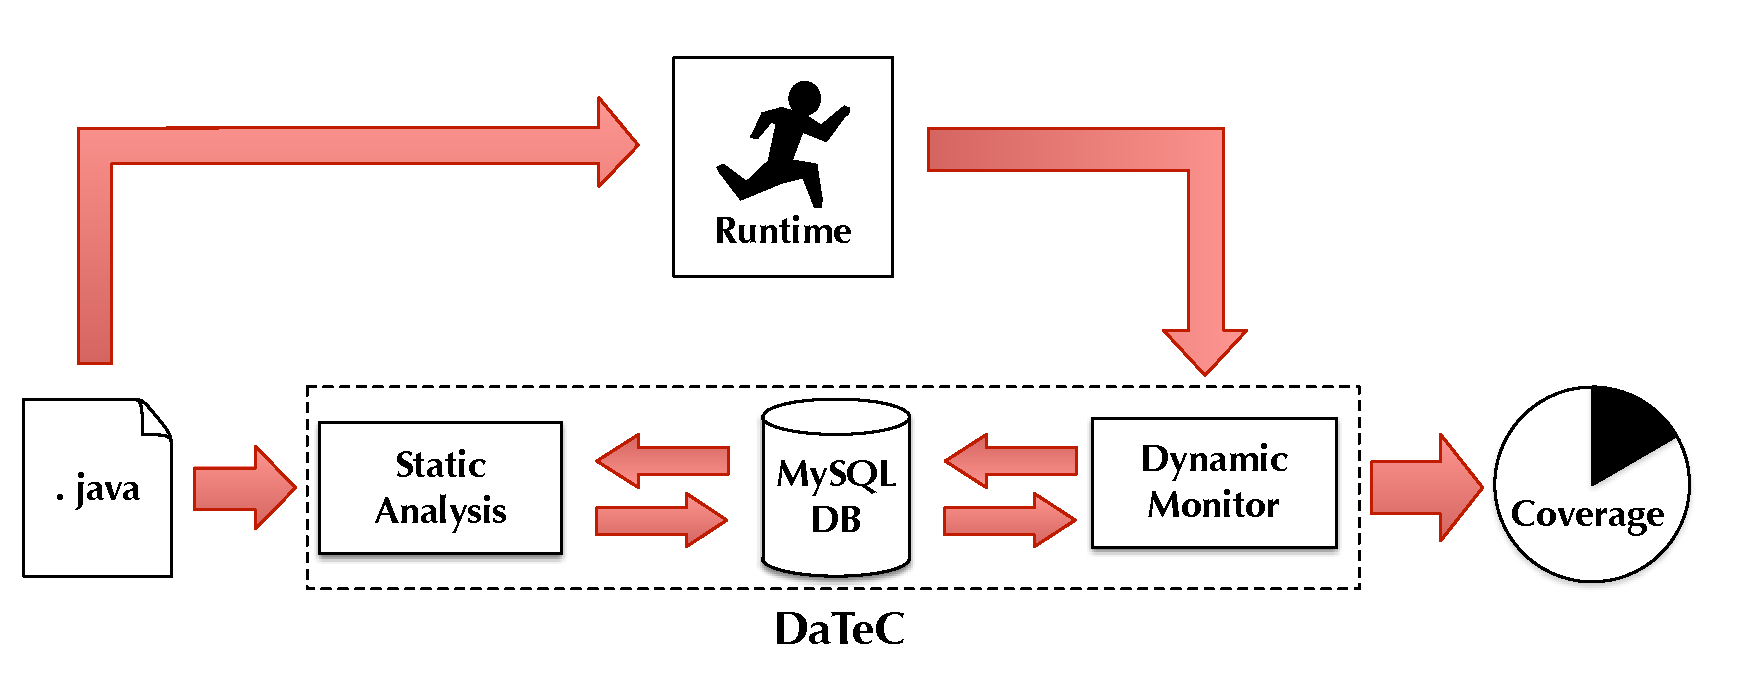
\includegraphics[width=\textwidth]{./Images/implementation.pdf}
   \caption{Implementation of the data flow testing tool}
  \label{implem}
  \end{center}
 \end{figure}

\subsection{Overview} 
The Dynamic Monitor performs three main steps to compute the data flow coverage of a given test suite:  
\begin{enumerate}
  \item Reads and interprets the data flow test objectives identified by the static analysis from the database;
  \item Instruments the program under analysis and dynamically monitor the execution to identify covered definition-use pairs;
  \item Updates the coverage information of the data flow test requirements identified statically and return a final report of the execution.
\end{enumerate}

\paragraph{}
The dynamic monitor exploits modular design (Figure \ref{modules}). 
\textit{StaticDB Interface} carries out the import and manipulation of the static analysis results. \textit{Active Fields Manager} instruments the program and monitors covered definition-use pairs. Finally, \textit{Report Manager} handles the presentation of the results in a format chosen by the user.
The role of each module will be discussed in relation to the function it carries out in the next sections.

 \begin{figure}[H]
   \begin{center}
   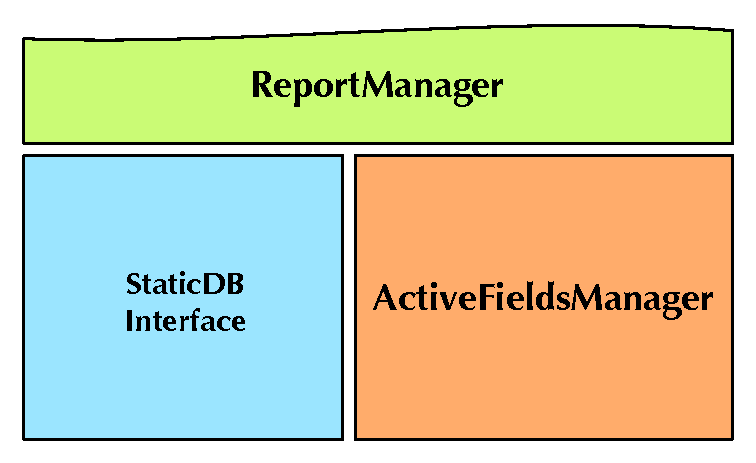
\includegraphics[scale=0.5]{./Images/phases.pdf}
   \caption{Modules of the Dynamic Monitor}
  \label{modules}
  \end{center}
 \end{figure}

\newpage
\subsection{Static analysis results management} 

\paragraph{}
The StaticDB Interface module performs the first step in the computation of the dynamic coverage, that is, the import of the results of the static analysis performed by \datec. In order to maintain an high degree of flexibility, I wanted to represents definitions, uses and associations between pairs as objects that could allow easy and clear comparison and retrieval. 

\paragraph{}
This was the main challenge in the implementation of this component, because the format in which the data is saved into \datec's database is less refined than what I needed to create object from it right away.
More specifically, \datec\ stores the results of the analysis in a MySQL database, in three tables: one for variable definitions, one for uses, and one for the associations defining the pairs. For each field, the 
name, the class, and the \textit{context} (i.e., the chain of methods that leads to a definition/use)  are stored as raw strings:

\begin{table}[H] 
  \centering
    \begin{tabular}{l|l}
    \textbf{completeName} & \textbf{defContext} \\ \hline
    \texttt{<inits.Foo: int i>}  &  \texttt{<inits.SubFoo: void <init>(int)>[8]<inits.Foo: void <init>()>[9]}        
    \end{tabular}
    \caption{An example row of the definitions table}
    \label{table:a_def}
\end{table}

\paragraph{}
The example of Table \ref{table:a_def} illustrates the definition of field \texttt{i} 
of type \texttt{int} belonging to class \texttt{inits.Foo}. This field has been 
assigned a value through means of the constructor of class 
\texttt{inits.SubFoo}, which, at line 8, calls the constructor of class 
\texttt{inits.Foo}. The actual definition occurs at line 9 of this constructor. 

\paragraph{}
As this format is not ideal for manipulation in a complex OO program, I needed to complement the import of data with additional parsing functionalities. This choice was enforced by the fact that \datec\ uses canonical method signatures, while the tool I exploited to perform dynamic instrumentation (see Section \ref{disl})  provides the informations about traced methods in the compact JVM format\footnote{\url{http://docs.oracle.com/javase/1.5.0/docs/guide/jni/spec/types.html\#wp276}}. In light of these limitations, the most convenient course of action was to parse data imported to the database, and transform it accordingly.

\begin{center}
\begin{jcode}[caption={Examples of transformation from canonical to compact form.}]
inits.SubFoo: void <init>(int) => inits/SubFoo: <init>(I)V
inits.Foo: boolean bar(String[],int) => inits/Foo: bar([Ljava/lang/String;I)Z
\end{jcode} 
\end{center}

\paragraph{}
In order to do so I implemented two interfaces, \texttt{FieldParser} and \texttt{MethodParser}. The database interface passes to \texttt{FieldParser} one row at a time; the parser creates a \texttt{Field} object out of it, and delegates to \texttt{MethodParser} the manipulation of the field's context. \texttt{MethodParser} uses a combination of regular expressions and the Guava Libraries\footnote{\url{https://code.google.com/p/guava-libraries/}} to manipulate the context raw string and transform it in a list of \texttt{Method} objects, in order to guarantee good performance. As I import the data, I also create create a \texttt{ContextGraph}. The \texttt{ContextGraph} is a \textit{multigraph} (i.e., a graph in which more than one edge between two nodes is allowed) where each node represents a method of the analyzed program in which at least one definition or one use takes place; it is implemented as a multigraph because there could be multiple call relationships between two methods. The nodes contain all the definitions/uses that occur in that method, and they are connected by directed, valued edges that contain the line number at which the destination method is called. This will be useful at the time of identification of the active fields.

\begin{figure}[H]
  \begin{center}
   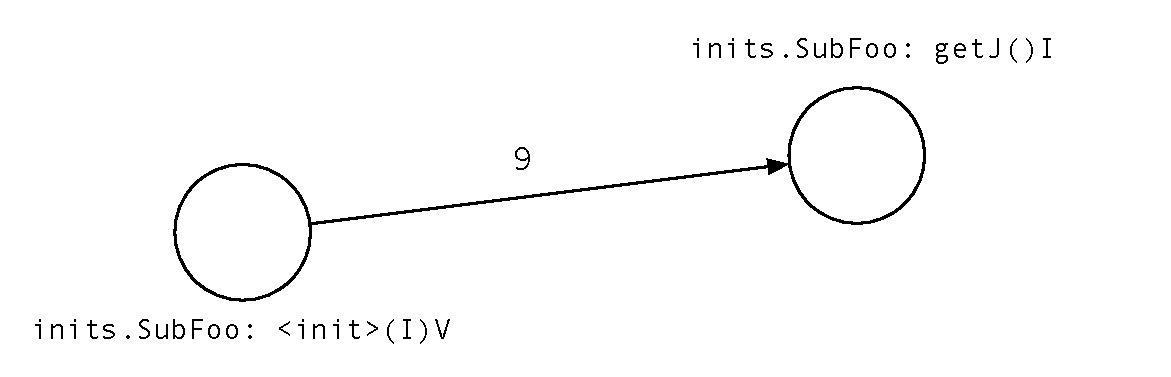
\includegraphics[scale=0.5]{./Images/graphexample.pdf}
   \caption{Example: the constructor of class \texttt{SubFoo} calls method \texttt{getJ} at line 9.}
  \label{gex}
  \end{center}
 \end{figure}

\paragraph{}
This implementation also accounts for the fact that the Static Analysis component is still a work in progress, and, as such, the format of the database may change: the aforementioned interfaces are implemented in two classes, \texttt{DatecFieldParser} and \texttt{DatecMethodParser}, which can parse the current version of the database output. Nevertheless, if a different version was needed, it would be enough to write new classes implementing the interested interfaces and specify their name in the tool's properties. The tool will then take care of exploiting the specified implementation through reflection.

\paragraph{}
For this part, the last concern was performance, because connecting to a database to retrieve the data and then parse it are resource intensive and time consuming operations, even when done efficiently. Moreover, there could be cases in which a user could perform more than one test on the same Java program. In this case, performing again the static analysis and manipulation would be a useless waste.
I addressed this concern by implementing an \texttt{Extractor} class: the class delegates to the database interface the import and manipulation of the data, and then serializes the produced collections. In case that the data in the database is not updated, \texttt{Extractor} avoids estabilishing a connection to the database, and just deserializes the existing data, resulting in increased efficiency.

\subsection{Dynamic instrumentation and coverage}
 
 The Active Fields Manager module implements the logic for the main task of the component, the computation of the data flow coverage achieved by a given test suite. To achieve the task, this module carries out several computations. 
First of all, the module must be able to instrument the program under test in the critical points to trace not only definitions and uses of fields, but also the chain of methods that define their context. 
Secondly, the module has to identify at runtime which definitions and which uses are active and which are killed, so that covered pairs can be properly identified. After the identification of all covered pairs, the third module will take care of generating a report.

\subsubsection{Dynamic instrumentation}\label{disl}
In order to instrument the program in the interested points, I defined four events: definition of a field, use of a field, basic block entry and basic block exit. These events are implemented in four methods of class \texttt{Recorder}:

\begin{itemize}
  \item \texttt{public void onBasicBlockIn(...)} is called upon entry in a basic block;
  \item \texttt{public void onBasicBlockOut(...)} is called upon exit from a basic block;
  \item \texttt{public void onInstanceFieldPut(...)} is called upon definition of a instance field;
  \item \texttt{public void onInstanceFieldGet(...)} is called upon use of a instance field.
\end{itemize}

\paragraph{}
These events acts as a layer on top of the tool I decided to use to capture information at runtime. This choice played a big role, as the component that collects runtime information is the critical part of the coverage computation tool in terms of 
performance; thus, it had to be performed carefully. I was presented with three 
popular solutions to trace the execution of a program in Java:
\begin{enumerate}
  \item Use low level instrumentation libraries (e.g. ASM);
  \item Use Aspect Oriented Programming libraries;
  \item Exploit the Java Debug Interface (JDI);
\end{enumerate}

\paragraph{}
The first solution offers the best performance, but at the same time is the most 
complex to use. The alternative solutions are simpler to use, but their performance are not as good as with ASM. 
Apart from the aforementioned approaches, recently researchers at USI proposed another technique for collecting runtime information of a program called \disl~\cite{Marek}.
 
\paragraph{}\label{eventhandler}
 \disl\ is a framework for dynamic analysis that acts as a middleware between ASM and the user, allowing the definition of 
 simple instrumentation rules through Java annotations, while also promising 
 performance levels higher than those offered by aspect oriented programming and JDI. \disl\ offers
 several predefined templates for instrumentations that I exploited for the analysis. 

\paragraph{}
More specifically, the annotation describes the point in which \disl\ performs code injection. Several parameters can be passed to the annotation, in order to define context information for the instrumentation. I illustrate how \disl\ works using the example reported in Listing~\ref{disl_snippet} that instrument all field definitions. This annotation injects code after (\texttt{@AfterReturning}) the bytecode region specified by the \texttt{BytecodeMarker} \textit{marker}, which in this case captures the allocation of new objects. The annotation \texttt{PutGuard} allowed me to define special \textit{guard} rules to filter out from the instrumentation objects I'm not interested in. Similarly, I specify a \textit{scope} useful to restrict the instrumentation to specific packages. Finally, \disl\ provides informations about the context of the instrumented code region through several parameters: I exploit \texttt{LineNumberStaticContext}, \texttt{FieldStaticContext} (providing \texttt{fieldName(), isArray(), isPrimitive()\dots}),  \texttt{MethodStaticContext} (providing \texttt{thisMethodName(), isPublic()\dots}) and \texttt{DynamicContext} to access context informations and use them to match the information with the one computed by the static analysis. 
  
 \begin{center}
 \begin{minipage}{0.8\textwidth}
    \begin{jcode}[caption={Instrumentation of definitions with DiSL}, label={disl_snippet}]
    @AfterReturning(marker = BytecodeMarker.class, args = "putfield", 
    guard = PutGuard.class, scope = Properties.SCOPE, order = 100)
    public static void afterRetPutField(LineNumberStaticContext lnsc, 
    FieldStaticContext fsc, MethodStaticContext msc, DynamicContext dc)
    { 
        EventHandler.instanceOf().onInstanceFieldPut(...);
    }
    \end{jcode} 
 \end{minipage}
\end{center}

\paragraph{}
Each \disl\ event corresponds to a call to different methods of the \texttt{EventHandler} interface. This interface acts as a communication layer between \disl\ annotations and the four events I defined in the class \texttt{Recorder}. In this way, the tool remains independent from the dynamic instrumentation technology chosen. 

\subsubsection{Coverage}

\paragraph{}
To compute data flow coverage at runtime, the tool must be able to trace which definitions are active or get killed during the execution, and match active definitions with executed uses. This means that, when a definition or a use occurs, the interested field has to be considered active, and the context in which the event occurred has to be registered. As the definition could be subsequently killed before its usage, in order for the coverage to be computed correctly, only the last definition must be marked as active. (Listing \ref{def},\ref{kill}) 

\begin{minipage}{0.5\textwidth}
\begin{jcode}[caption={Variable median is defined (line 5).},label={def}]       
public class MathOps {
  private float median;
  
  public MathOps(){
    median = 0;
  }
  
  ...
}    
\end{jcode} 
\end{minipage}
\begin{minipage}{0.5\textwidth}
\begin{jcode}[caption={Variable median is redefined (line 6): this definition kills the previous one.},label={kill}]       
public class MathOps {

  ...
  
  public void getMedian(...){
    median = computeMedian(...);
    return median;
  }
}  
\end{jcode} 
\end{minipage}

\paragraph{}
In order to easily identify active definitions and uses, the implementation exploits the \texttt{ContextGraph} built at import time. 
When I enter (or exit from) a basic block, I move accordingly in the graph, checking that the line number corresponds to the value of the edge and the destination node signature is the same as the destination basic block instrumented. On the other hand, when a definition or a use occurs, I match it against the static definition and uses present in that node, exploiting two informations: the field's name and the context. The context, that is the chain of methods which led to the definition or use, is obtained by tracking the traversed path inside the graph with a stack of the nodes: whenever I enter a method I push it in the stack, and whenever I exit from it I pop it. These two informations are enough to univocally identify the field. 

 \paragraph{}
 The following step consists in marking the definition/use as active. In order to do so, I needed to track not only informations about the field and its context, but also identify the object that produced it. Otherwise, I could incorrectly cover some pairs that where not actually executed. In addition, I needed some data structure that could allow me to write and retrieve active fields with little overhead. I achieved these objectives by implementing the main interface of this module, \texttt{ActiveFieldsManager}, which manages the registration of active definitions and uses in two \texttt{ActiveFieldMap}s. An \texttt{ActiveFieldMap} is like a Java \texttt{Map}, except from the fact that it supports not only 1-to-1 relationships, but also 1-to-many. This is due to the fact that in the same objects there could be many different definitions and uses.
 
\paragraph{}
When the tool registers a field's definition or use, it records it in the proper \texttt{ActiveFieldMap} with a mapping Object~$\rightarrow$~(Field, Context). Objects are uniquely identified by exploiting their \texttt{identityHashCode}\footnote{\url{http://docs.oracle.com/javase/7/docs/api/java/lang/System.html\#identityHashCode(java.lang.Object)}}. This implementation allows me to quickly register fields as active under one object's \texttt{identityHashCode}, and also kill them by overwriting them.

\paragraph{}
Furthermore, the tool currently implements two different ways of marking fields as active: the tool can either perform a standard coverage, or alternatively perform a wider coverage by taking into account fields' definitions/uses which are implicitly covered:

\begin{table}[H] 
  \centering
    \begin{tabular}{l|l}
    \textbf{completeName} & \textbf{defContext} \\ \hline
    \texttt{<inits.Foo: int i>}  &  \texttt{<inits.SubFoo: void <init>(int)>[8]<inits.Foo: void <init>()>[9]} \\ 
    \texttt{<inits.Foo: int i>}  &  \texttt{<inits.Foo: void <init>()>[9]}        
    \end{tabular}
    \caption{Two definitions of the same field. The second definition can be implicitly covered.}
    \label{table:implicit}
\end{table}

\paragraph{}
In the example from Table \ref{table:implicit}, the second definition can be implicitly covered in case the first 
definition is covered; this behavior can improve the coverage extension. The two different methods are provided through two subclasses  of \texttt{ActiveFieldMap}: \texttt{SimpleActiveFieldMap} and \texttt{SubsumeActiveFieldMap}. The user can specify the preferred behavior by tweaking the tool's properties, and the appropriate implementation will be chosen at runtime.

\paragraph{}\label{associations}
The last step in the computation of the coverage is the marking of definition-use pairs as covered. A marking occurs after the registration of a use as active, because in that case I can safely assume that there is a corresponding active definition. The class \texttt{Associations} contains all the possible definition-use pairs imported from the static analysis, paired with a boolean that mark the pair as covered or not covered. Whenever I register an active use, I retrieve the corresponding active definition (matching by object's \texttt{identityHashCode} and field name),  and mark it as active by switching the boolean value to true. In addition, \texttt{Associations} keeps track of the amount of total pairs in the collection, and the amount of covered pairs. %Finally, the class supports simple iteration provided by two methods: method \texttt{next()}, which returns a tuple composed of (Field, defContex, useContext), and method \texttt{hasNext()}, which tells if there are more tuples to process in the collection. These two methods are useful in the generation of the final report. %questo perzzo � inutile

\subsection{Report generation and presentation of final results}

\paragraph{}
One of the requirements for the tool was the generation of a final report containing the results of the produced coverage. I wanted the user of the tool to be able to create custom report that could suit his needs easily, and without changing the tool's code. 

\paragraph{}
I met this requirement by implementing an \texttt{OutputManager} interface, which features one method: \texttt{write(Associations~a)}. If a user wanted to generate a report in a format different from what is already provided, it would be enough to create a new class implementing the \texttt{OutputManager} interface; this process should be quite straightforward, as I also provide an easy way to iterate through the pairs (see Section \ref{associations}). 

\paragraph{}
As of today, the tools supports two ways of generating a report: either printed to the standard output (this was mainly useful to me for debugging and testing purposes), or saved in a report in XML format. The user can specify the preferred format by switching the dedicated property in the tool's properties, in form of the complete class name in which the report generation is implemented.

\paragraph{}
As an example, the following listing contains a simple report printed to the standard output, which indicates from what database the static analysis informations were extracted, which classes were used to parse it, and which class was used to generate the report.
 
 \newpage
\lstset{basicstyle=\ttfamily}
\begin{jcode}[caption=Example of the application output]
Application is starting.
Database datecm will be parsed according to these classes:
[FIELDPARSER]: ch.usi.star.datec.coverage.context.DatecFieldParser
[METHODPARSER]: ch.usi.star.datec.coverage.context.DatecMethodParser
Results will be presented according to class: 
[OUTPUTSINK]: ch.usi.star.datec.coverage.utilities.StdOut

Db is up to date, reading defs from serialized FieldMap...
Successfully read from serialized StaticFieldMap
Db is up to date, reading uses from serialized FieldMap...
Successfully read from serialized StaticFieldMap
Db is up to date, reading associations from serialized Map...
Successfully read from serialized associations

Application has finished computing coverage.

Time elapsed: 393 ms.
COVERED PAIRS: (3 out of 5)
[Field] <inits.SubFoo: int j> [D]: [inits.SubFoo: setJ(I)V[12]] [U]: [inits.SubFoo: getJ()I[14]] [COVERED]: true
[Field] <inits.SubFoo: int j> [D]: [inits.SubFoo: <init>(I)V[9]] [U]: [inits.SubFoo: getJ()I[14]] [COVERED]: true
[Field] <inits.Foo: int i> [D]: [inits.Foo: setI(I)V[14]] [U]: [inits.Foo: getI()I[12]] [COVERED]: false
[Field] <inits.Foo: int i> [D]: [inits.SubFoo: <init>(I)V[8], inits.Foo: <init>()V[9]] [U]: [inits.Foo: getI()I[12]] [COVERED]: true
[Field] <inits.Foo: int i> [D]: [inits.Foo: <init>()V[9]] [U]: [inits.Foo: getI()I[12]] [COVERED]: false

Shutdown...
\end{jcode}


\section{Verification}\label{validation}

The last phase of this Bachelor Project consisted in the verification of my tool against its requirements. 
The verification of the complete version of \datec~was challenging: to assess the correctness of my implementation it is necessary to check wether the data flow coverage of a test suite identified by \datec~corresponds to the actual set of definition-use pairs that were executed by the test suite itself. This process cannot be automated and therefore is particularly time consuming because it requires to manually inspect both the test cases and the executed software. 

Since performing this manual check on large numbers of test cases is impossible for time constraints, I organized the verification activity in two steps: at first, I designed a set of specific test cases of limited size to check corner cases, on which I checked in details each covered and not covered definition use pairs; and then in a second step I performed sample checks on coverage obtained executing large test suites on open source projects. 

In the next sections I'm describing the checked requirements and these two steps of verification activity that I performed. 


%This process was nontrivial for a number of reasons: first, we had to establish the metrics that we were interested to measure during the evaluation; secondly, before actually testing the tool with projects and test suites of considerable size, I wanted to make sure that the tool produced the expected results for small-sized samples. The reason for this choice is that the Dynamic Monitor relies heavily on the results of the static analysis, and, more importantly, on the runtime instrumentation informations provided by \disl. If these informations did not match the expectations, there could have been errors in the final results. For this reason, the evaluation of the tool was divided in two phases: at first, I created and executed small ``sanity check" test cases. In a second moment, I tested the tool with a bigger project.

\subsection{Requirements}
I evaluated \datec~correctness and performances. I consider \datec~to be correct wether the identified coverage corresponds to the actual coverage obtained during the execution. To check the correspondance, I performed manual checks inspecting the code of the test cases and of the applications. 

Regarding performances, I focused on time constraints. I measured the total amount of time required to execute a test suite together with \datec~, and the overhead caused by the dynamic monitoring. To compute the overhead, I compared the execution time of a test suite executed with \datec~ against its original execution time. The evaluation of the performance was carried on to verify that the tool was actually usable (e.g. it did not require weeks of execution) on medium-big size java projects.%, I was not provided with a specific overhead threshold.  
Since I was not provided with a specific overhead threshold, the evaluation doesn't provide for a formal efficiency statement. 
 
\subsection{Preliminary tests}
The first step in the evaluation was the creation and verification of small test cases. I used these test cases to check that the tool behaved as expected. I wanted to make sure to cover some nontrivial cases that could occur while programming in Java. To this purpose, I wrote a test organized in packages, where each package would represent one corner case. Afterwards, I ran these tests and checked that the results were as expected. Time was not a concern for this test cases, because of their marginal size. In Table \ref{table:minitest}, I present the most relevant of these test cases; each one covers one specific feature of Java programming.

\begin{table}[H] 
  \centering
    \begin{tabular}{|l|p{0.6\textwidth}|}
    \hline
   \textbf{Package Name} & \textbf{Test Case Description}\\ \hline
      \texttt{arrays}  &  Instrumentation of array load and store events. Tests array creation and index access.\\ \hline
      \texttt{inits}  &  Instrumentation of constructors. Tests abstract classes and uses of \texttt{super()}\\ \hline
      \texttt{nested}  &  Instrumentation of nested classes. Mainly used to check correct parsing of class names (e.g \texttt{package.Class\$NestedClass}) and bytecode generated fields (e.g., \texttt{this\$0})\\ \hline
      \texttt{staticinits}  &  Instrumentation of static constructors (e.g., Singleton Pattern \texttt{instanceOf()}) \\ \hline
    \end{tabular}
    \caption{Preliminary tests}
    \label{table:minitest}
\end{table}

\subsection{Testing a real life use case}

\subsubsection{Choosing the software to be tested}

After checking that the results of the preliminary tests were correct, I tested the tool with a more complex software, in order to simulate a real use case of the tool. In order to do this, I had to find a Java software which would be bigger than the average student projects I used to test before. In addition, the software would have to be an attached test suite big enough to cover a number of cases.

\paragraph{}
After some research, I chose to test my tool with JGraphT\footnote{http://jgrapht.org/}, a Java library that provides graph theory objects and algorithms. JGraphT features more than 150 classes, and comes with attached JUnit test cases which test every feature of the library. In the first place, I tested the coverage of each test case separately, to measure the time of execution of the coverage and the quality of the coverage (the number of pairs covered) of a single test case. On a second time, I ran the tool on all the test cases at once.

\subsubsection{Performing the evaluation}

I split the evaluation in two phases: in the first, I would test the coverage computation on each single test case separately, to assess the average coverage of each one; secondly, I would run the tool with all the test cases at once, to assess the overall coverage and the performance of the tool with a big input. For both phases, I would keep track of the amount of time used by the tool, and the \textit{all DU pairs coverage} (Section \ref{criteria}) measurement. Overall, I ran the tool on a total of 80 JUnit test cases.


\subsubsection{Results}

The Static Analysis component registered a total of 10147 possible definition-use pairs. Nevertheless, running each test case separately covered on average 50 definition-use pairs (see Figure \ref{results}). Evaluation of the time factor showed that the tool is quite efficient, since each the execution and coverage computation of each test case took on average 3-5 seconds. It puts a significant overhead on the execution of the test cases, since each test case executed without analysis terminates in \textasciitilde100-400 ms. Anyway, it can be considered acceptable.

\paragraph{}
Running all the test cases at once (158 tests) showed that the test cases cover a small range of definition-use pairs, which are exercised many times: in fact, only 289 pairs were covered, but the number would raise if counting the coverage of the same pair more than one time. The tool computed the coverage in roughly 153 seconds.

\newpage

\begin{figure}[htb]
  
\centering
%\centering
%\makebox[0pt][c]{%
%\begin{minipage}[b]{1\linewidth}
%\centering
  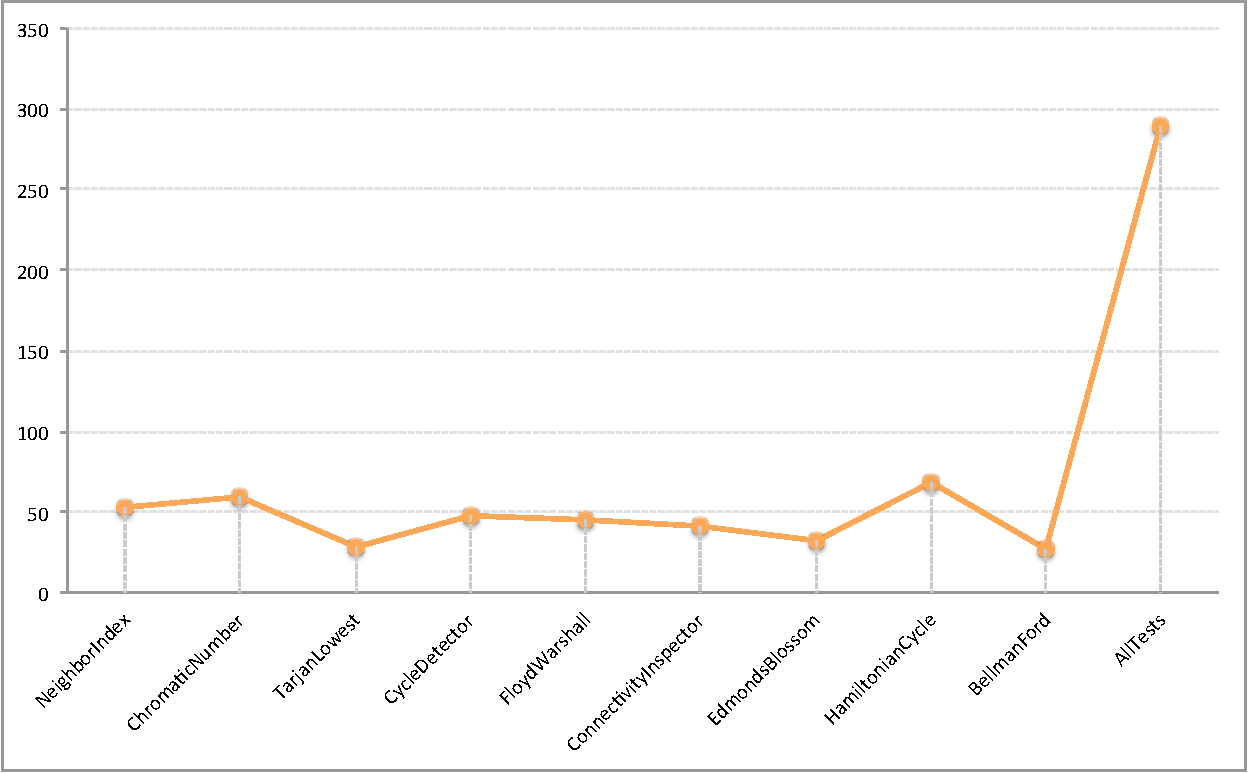
\includegraphics[width=0.8\textwidth]{./Images/tests.pdf}
  \caption{Coverage results of 10 random test cases.}
\label{results}
%\end{minipage}%
%\hspace{0.1cm}
%\begin{minipage}[b]{1\linewidth}
%\centering
% 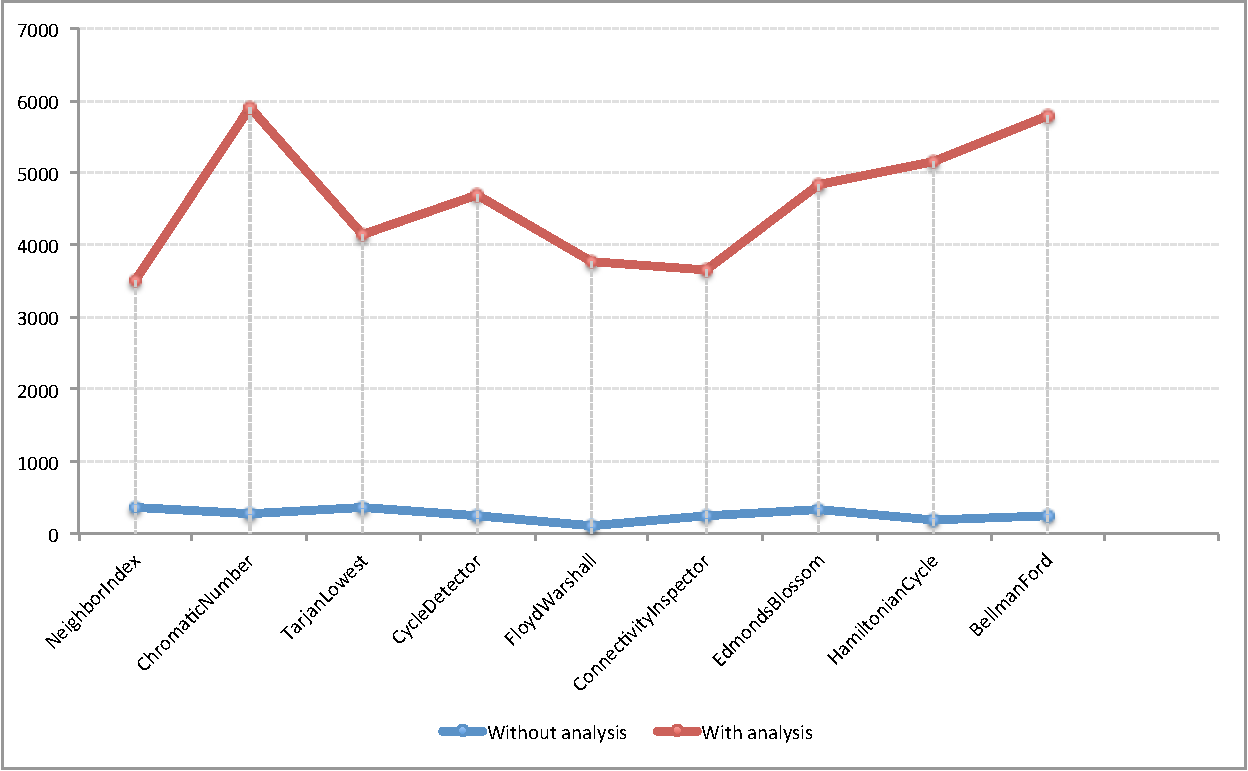
\includegraphics[width=0.95\textwidth]{./Images/overhead.pdf}
% \caption{Time overhead.}
%\label{time}
%\end{minipage}%
%}%

\end{figure}



%\begin{minipage}{0.5\textwidth}
%\begin{figure}[H]
%  \begin{center}
%   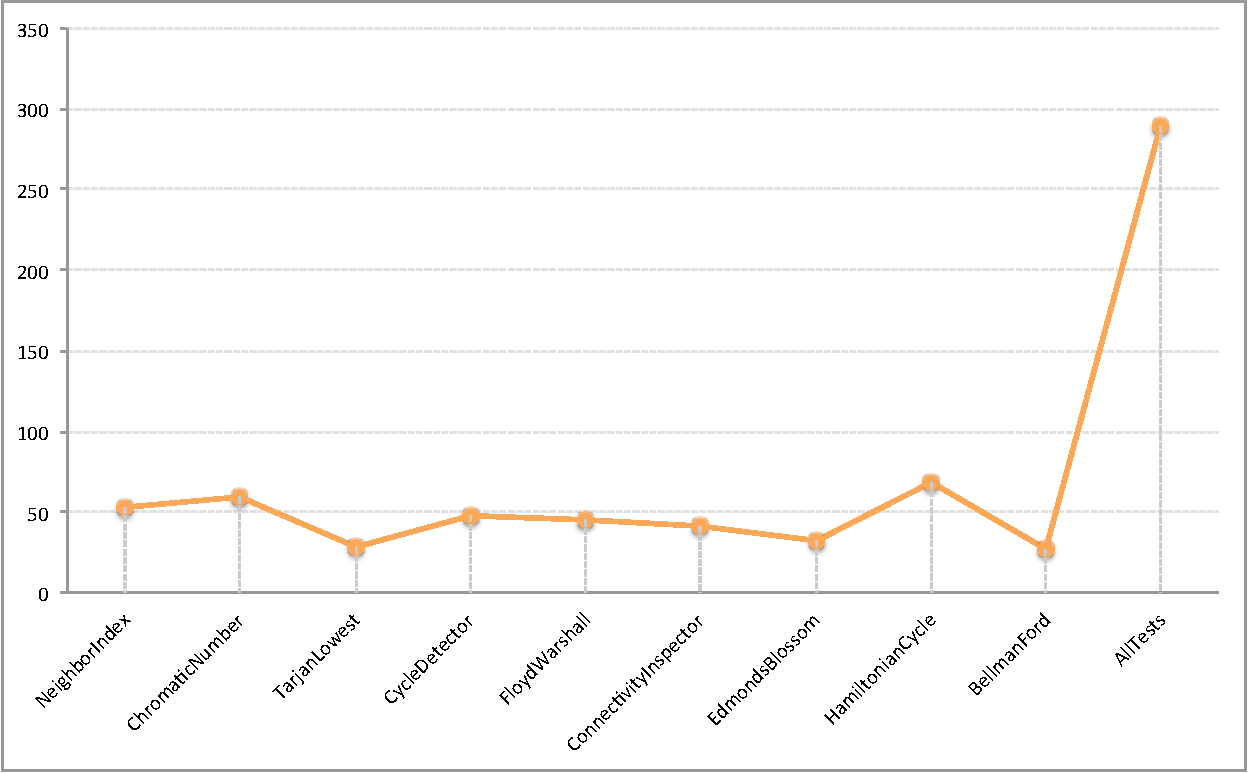
\includegraphics[width=\textwidth]{./Images/tests.pdf}
%   \caption{Coverage results of 10 random test cases.}
%  \label{results}
%  \end{center}
% \end{figure}
% \end{minipage}
% \begin{minipage}{0.5\textwidth}
%\begin{figure}[H]
%  \begin{center}
%   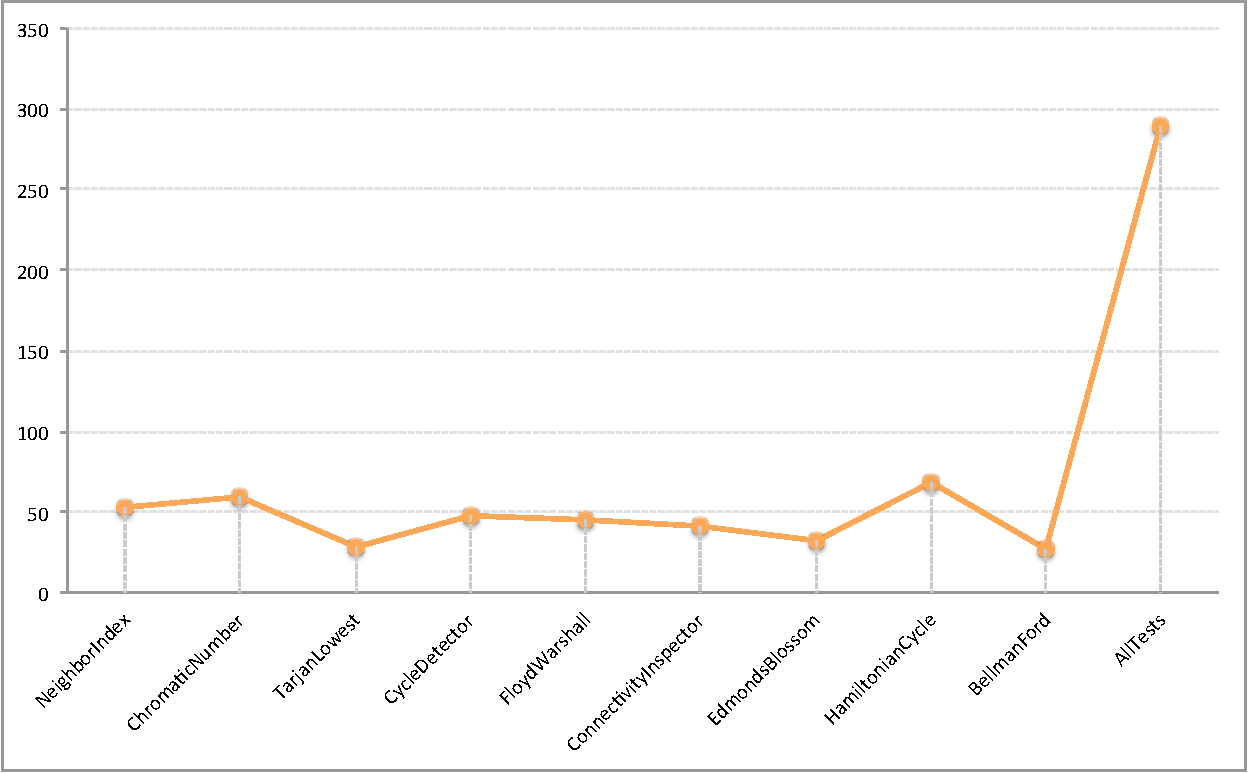
\includegraphics[width=\textwidth]{./Images/tests.pdf}
%   \caption{Coverage results of 10 random test cases.}
%  \label{results}
%  \end{center}
% \end{figure}
% \end{minipage}

%% menzionare che certe coppie non vengono calcolate?
\begin{figure}[htb]
  
\centering
%\centering
%\makebox[0pt][c]{%
%\begin{minipage}[b]{1\linewidth}
%\centering
%  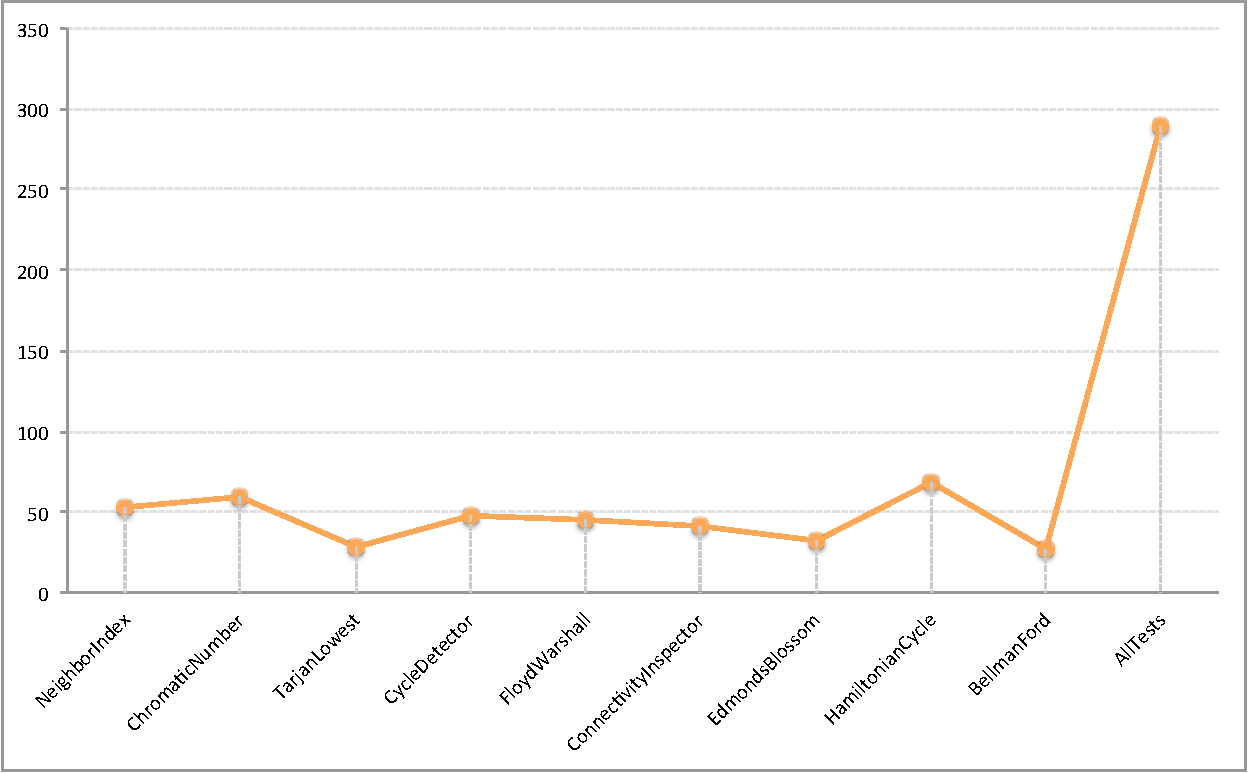
\includegraphics[width=0.6\textwidth]{./Images/tests.pdf}
%  \caption{Coverage results of 10 random test cases.}
%\label{results}
%\end{minipage}%
%\hspace{0.1cm}
%\begin{minipage}[b]{1\linewidth}
\centering
 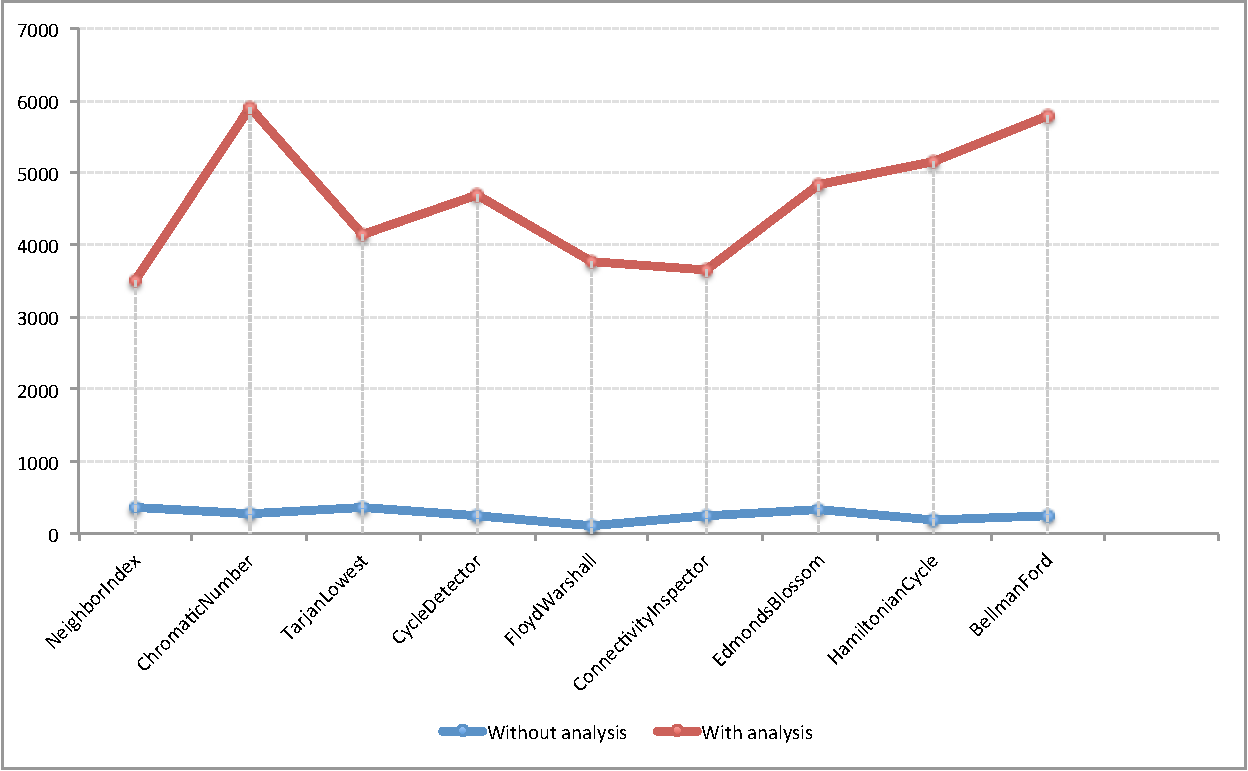
\includegraphics[width=0.8\textwidth]{./Images/overhead.pdf}
 \caption{Time overhead.}
%\label{time}
%\end{minipage}%
%}%

\end{figure}




\section{Conclusions}\label{conclusions}
%Timeline
\paragraph{}
In this project I developed a dynamic monitor for a data flow testing tool, and performed an evaluation to assess its efficiency and its effectiveness. Given the good performances of the tool, I will publish it online to help researchers and practitioners experimenting with data flow criteria --- it could be used for collecting new data on the effectiveness of data flow criteria, or it could be extended with a component that automatically generates test cases for the missing pairs for defining new test case generation approaches. 

\paragraph{}
I was impressed by the low coverage observed on the test suites that I used in the evaluation phase. This suggests that data flow testing is still an open problem that needs new data and techniques, and that provide a complementary view with respect to functional testing and simpler structural criteria like branch and statement testing. 

\paragraph{}
Apart from the results obtained, this project was an invaluable opportunity for me, because it allowed me to apply some concepts I learned during my Bachelor and I had never truly applied before, especially regarding programming principles and design patterns. I learned to write code that can be reused and modularized, and the importance of careful design and planning. Moreover, since I was left a lot of freedom during the development, for the first time I had to learn how to organize the time I could dedicate to the project, and how to use it effectively. The experience I collected from this Bachelor project will be extremely useful in future occasions.

\section{Acknowledgements}
First of all, I would like to thank my advisor Prof. Mauro Pezz\'e for providing me this opportunity. Exploring and working on an unknown topic was a precious experience, and will be very helpful during my future studies. I would also like to thank Mattia Vivanti, which supervised me during the whole project and has always been very helpful and has given me a lot of precious advices. Last but not least, I would like to thank my parents, my girlfriend and my friends for being supportive throughout these three years.


\newpage
\bibliographystyle{abbrv}
\bibliography{references}

\end{document}
